\documentclass{beamer}
\usetheme{metropolis}
\usepackage{graphicx}
\usepackage{subfig}
\usepackage{tcolorbox}
\title{Calculus-Based Physics-2: Electricity, Magnetism, and Thermodynamics (PHYS180-02): Unit 5}
\author{Jordan Hanson}
\institute{Whittier College Department of Physics and Astronomy}

\begin{document}
\maketitle

\section{Unit 4 Review}

\begin{frame}{Unit 4 Review}
Suppose a bundle of wires is carrying current along what we call the $\hat{z}$ direction.  Each wire runs along the z-axis and they are close enough to ignore the fact that the volume of each wire prevents it from being exactly on the z-axis.  One wire carries +2.0 A, another carries +1.5 A, and a third carries -0.5 A.  What is the B-field strength at a distance of 1 cm away in the x-y plane?
\begin{itemize}
\item A: 6 Gauss
\item B: 0.6 Gauss
\item C: 6 Tesla
\item D: 0.6 Tesla
\end{itemize}
\end{frame}

\begin{frame}{Unit 4 Review}
Suppose a loop of current exists in the x-y plane, and a uniform B-field is in the $\hat{z}$ direction.  Which of the following will occur?
\begin{itemize}
\item A: The loop will not rotate - there is no torque.
\item B: The loop will rotate 180 degrees - there is torque.
\item C: The loop will rotate 90 degrees - there is torque.
\item D: The loop will rotate -90 degrees - there is negative torque.
\end{itemize}
\end{frame}

\section{Summary}

\begin{frame}{Summary}
\textbf{Reading: Chapters 13 and 14} \\ \vspace{0.5cm}
\begin{enumerate}
\item 13.1-2: Faraday's and Lenz's Law
\item 13.3: Motional EMF
\item 13.4: Induced E-fields
\end{enumerate}
\begin{enumerate}
\item 14.1: Mutual inductance
\item 14.2: Self-inductance and inductors
\item 14.3: Energy in a magnetic field
\end{enumerate}
\end{frame}

\section{Faraday's Law and Lenz's Law}

\begin{frame}{Faraday's Law}
\begin{figure}
\centering
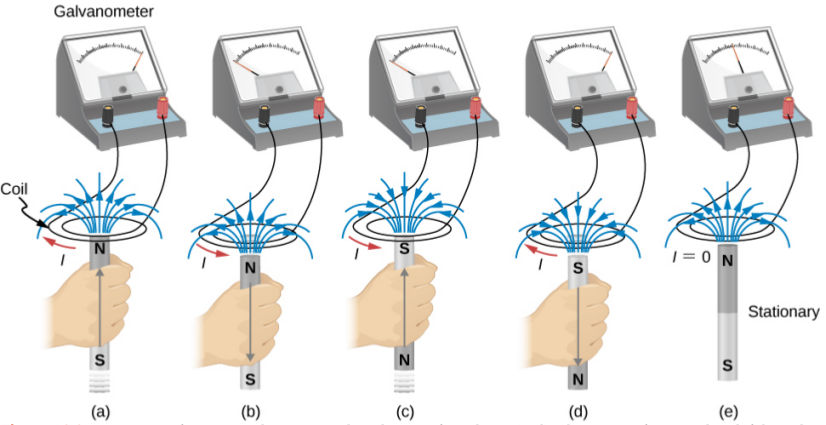
\includegraphics[width=0.9\textwidth]{figures/farad.png}
\caption{\label{fig:farad1} Not only does moving charge create B-fields, but B-fields can create moving charge.  Study each of the cases above, and (Professor) define the concept of \textit{magnetic flux}.}
\end{figure}
\end{frame}

\begin{frame}{Faraday's Law}
\begin{figure}
\centering
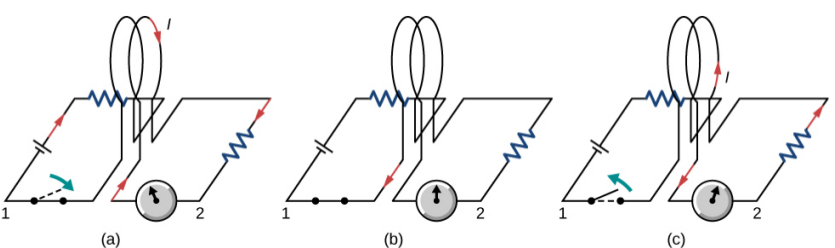
\includegraphics[width=0.9\textwidth]{figures/farad2.png}
\caption{\label{fig:farad2} In addition to a moving magnetic field, \textit{other circuits} can make current flow in a circuit.  The effect must have something to do with \textit{changing} magnetic fields.}
\end{figure}
\end{frame}

\begin{frame}{Faraday's Law}
\begin{tcolorbox}[colback=white,colframe=black!40!black,title=Faraday's Law]
\alert{The emf $\epsilon$ induced is the negative change in the magnetic flux $\Phi_m$ per unit time. Any change in the magnetic field
or change in orientation of the area of the coil with respect to the magnetic field induces a voltage (emf).
\begin{align}
\phi_m &= \int_S \vec{B} \cdot d\vec{A} \\
\epsilon &= - \frac{d\phi_m}{dt}
\label{eq:farad}
\end{align}}
\end{tcolorbox}
\textit{The unit of magnetic flux is the Webter, or 1 Wb = 1 T m$^2$.}
\end{frame}

\begin{frame}{Faraday's Law}
\small
\textbf{Example:}
A square coil has sides 0.25 m long and is tightly wound with 200 turns of wire. The resistance of the coil 5.0 Ohms. The coil is placed in a spatially uniform magnetic field that is directed perpendicular to the face of the coil and whose magnitude is decreasing by −0.040 T/s. (a) What is the magnitude of the emf induced in the coil? (b) What is the magnitude of the current circulating through the coil?
\begin{figure}
\centering
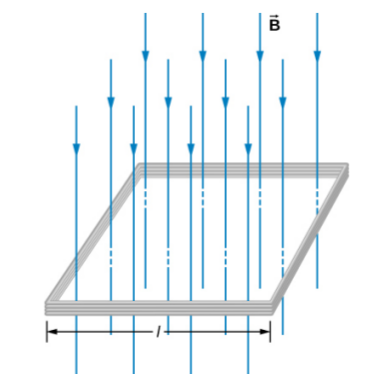
\includegraphics[width=0.3\textwidth]{figures/loop1.png}
\caption{\label{fig:loop1} A 200 turn loop in a B-field.}
\end{figure}
\end{frame}

\begin{frame}{Faraday's Law}
\begin{tcolorbox}[colback=white,colframe=black!40!black,title=Lenz's Law]
\alert{The direction of the induced emf drives current around a wire loop to always oppose the change in magnetic flux that
causes the emf.}
\end{tcolorbox}
\end{frame}

\begin{frame}{Faraday's Law}
\small
\textbf{Example:}
A magnetic field B is directed outward perpendicular to the plane of a circular coil of radius r = 0.50 m.  The field is cylindrically symmetrical with respect to the center of the coil, and its magnitude decays exponentially according to
\begin{equation}
B(t) = B_0 \exp(-a t)
\end{equation}
with $B_0 = 1.5$ T and $a = 5.0$ s$^{-1}$.  (a) Calculate the emf induced in the coil at the times $t_0 = 0$, $t_1 = 0.05$, and $t_2 = 1.0$ seconds. (b) Determine the current in the coil if the resistance is 10 Ohms. 
\end{frame}

\begin{frame}{Faraday's Law}
In the previous example, what would happen if the area $A$ of the loop were increased?
\begin{itemize}
\item A: The current would decrease.
\item B: The current would stay the same.
\item C: The voltage would decrease.
\item D: The voltage would increase.
\end{itemize}
\end{frame}

\begin{frame}{Faraday's Law}
In the previous example, what would happen if the sign of the exponent in $B(t)$ were flipped?
\begin{itemize}
\item A: The current would reverse direction and increase in magnitude.
\item B: The current would reverse direction and decrease in magnitude.
\item C: The current would keep the same direction and increase in magnitude.
\item D: The current would keep the same direction and decrease in magnitude.
\end{itemize}
\end{frame}

\begin{frame}{Faraday's Law}
In the previous example, what would happen if $\alpha$ in the exponent in $B(t)$ were increased?
\begin{itemize}
\item A: The current would reverse direction and increase in magnitude.
\item B: The current would reverse direction and decrease in magnitude.
\item C: The current would keep the same direction and increase in magnitude.
\item D: The current would keep the same direction and decrease in magnitude.
\end{itemize}
\end{frame}

\begin{frame}{Faraday's Law}
\small
\textbf{Example:}
The square coil of Figure \ref{fig:loop2} has sides l = 0.25 m long and is tightly wound with N = 200 turns of wire. The resistance of the coil is R = 5.0 $\Omega$. The coil is placed in a spatially uniform magnetic field that is directed perpendicular to the face of the coil and whose magnitude is decreasing at a rate $dB/dt = −0.040 t^2$. (a) Graph the magnitude of the emf induced in the coil. (b) What is the magnitude of the current through the coil at 100 ms?
\begin{figure}
\centering
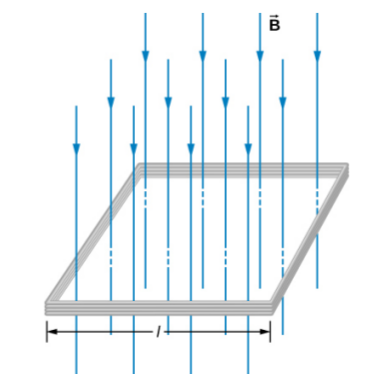
\includegraphics[width=0.3\textwidth]{figures/loop1.png}
\caption{\label{fig:loop2} A 200 turn loop in a B-field.}
\end{figure}
\end{frame}

\begin{frame}{Lenz's Law}
\begin{figure}
\centering
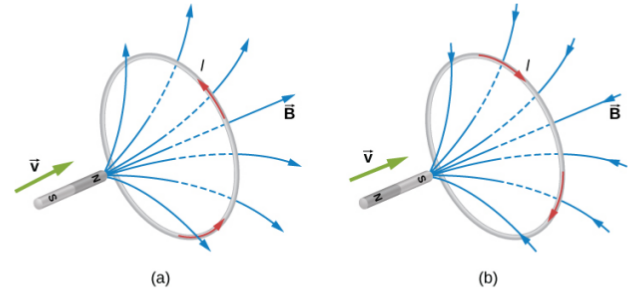
\includegraphics[width=0.8\textwidth]{figures/lenz.png}
\caption{\label{fig:loop3} Lenz's Law relates sign of current to B-field.}
\end{figure}
\end{frame}

\section{Motional EMF}

\begin{frame}{Lenz's Law}
\small
\begin{figure}
\centering
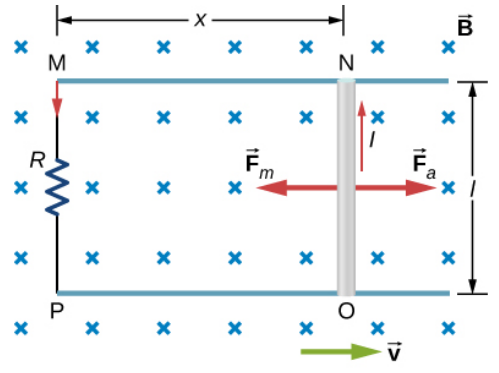
\includegraphics[width=0.5\textwidth]{figures/loop2.png}
\caption{\label{fig:loop4} A system in which the magnetic flux depends on time.}
\end{figure}
\begin{enumerate}
\item Show that power is equal to $P = \vec{F} \cdot \vec{v}$ for constant acceleration.
\item Show that the emf is $\epsilon = B l v$, from Faraday's Law.
\item Show that power generated, $P = I^2 R$, is equal to power injected.
\end{enumerate}
\end{frame}

\begin{frame}{Faraday's Law}
In the previous example, what would happen if $\vec{F}_a$ was pointed to the left?
\begin{itemize}
\item A: The current would reverse direction.
\item B: The current would keep the same direction.
\item C: The magnetic flux due to the external field would decrease.
\item D: A and C
\end{itemize}
\end{frame}

\begin{frame}{Faraday's Law}
In the previous example, what would happen if $R$ were increased, but the magnitude of $F_a$ were kept the same?
\begin{itemize}
\item A: The current would decrease.
\item B: The current would increase.
\item C: The current would remain constant.
\item D: The power required would increase.
\end{itemize}
\end{frame}

\section{Induced Electric Fields}

\begin{frame}{Induced Electric Fields}
Recall that the relationship between voltage and electric field is
\begin{equation}
\vec{E} = - \nabla V = -\frac{\partial V}{\partial x}\hat{x}-\frac{\partial V}{\partial y}\hat{y}-\frac{\partial V}{\partial z}\hat{z}
\end{equation}
In one dimension, this becomes
\begin{equation}
\vec{E} = -\frac{dV}{dx}\hat{x}
\end{equation}
If we take a dot product with $- d\vec{x} = - dx ~ \hat{x}$ on each side, we find
\begin{equation}
-\vec{E} \cdot d\vec{x} = dV
\end{equation}
Integrating, we have
\begin{equation}
V = - \int \vec{E} \cdot d\vec{x}
\end{equation}
\end{frame}

\begin{frame}{Induced Electric Fields}
However, if the voltage is a result of a changing magnetic field, and Faraday's Law, then
\begin{equation}
\frac{d\phi_m}{dt} = \oint \vec{E} \cdot d\vec{x}
\end{equation}
Recall that from \textit{electrostatics},
\begin{equation}
\oint \vec{E} \cdot d\vec{x} = 0 \label{eq:cons}
\end{equation}
Equation \ref{eq:cons} is true for eletrostatics because the Coulomb force is \textbf{conservative}.  But in a previous example we showed that power was being generated and \textit{conserved}, despite the fact that magnetic flux is changing.  What is happening?
\end{frame}

\begin{frame}{Lenz's Law}
\small
\begin{figure}
\centering
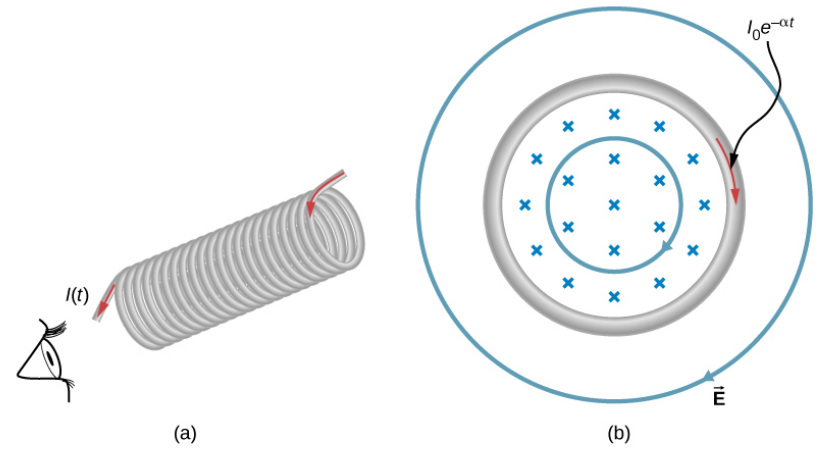
\includegraphics[width=0.7\textwidth]{figures/loop3.png}
\caption{\label{fig:loop5} A solenoid with a changing current will induce an E-field.  The solenoid has turn density $n$, and is long compared to the radius.}
\end{figure}
\begin{enumerate}
\item What is the E-field outside the solenoid?
\item What is the E-field inside the solenoid?
\item Create a graph of the E-field strength versus distance.
\end{enumerate}
\end{frame}

\begin{frame}{Faraday's Law: An application}
\small
\begin{figure}
\centering
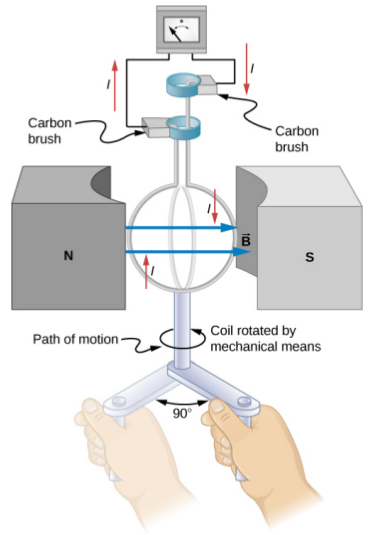
\includegraphics[width=0.33\textwidth]{figures/gen1.png}
\caption{\label{fig:gen1} The basic concept behind an AC generator.}
\end{figure}
\end{frame}

\begin{frame}{Faraday's Law: An application}
Start with Faraday's Law:
\begin{equation}
\epsilon = - \frac{d\phi_B}{dt}
\end{equation}
The flux $\phi_B$ is changing and depends on time:
\begin{equation}
\phi_B = \vec{B} \cdot \vec{A}(t) = BA\cos(\theta(t))
\end{equation}
Let the \textit{angular velocity} be constant: $\theta = \omega t$.  Then we have
\begin{equation}
\phi_B  = BA\cos(\omega t)
\end{equation}
Thus the emf (with $N$ loops) is
\begin{equation}
\epsilon = N\omega BA \sin(\omega t) = \epsilon_0 \sin(\omega t)
\end{equation}
\textbf{The generation of AC power stems from $\omega$.} \\ (Professor: diagram of $\epsilon(t)$).
\end{frame}

\begin{frame}{Faraday's Law}
\begin{equation}
\epsilon = N\omega BA \sin(\omega t)
\end{equation}
The AC voltage equation above is a basic model for the voltage from a generator.  Which of the following would increase the \textit{amplitude} of the emf?
\begin{itemize}
\item A: Turning the area more slowly.
\item B: Turning the area more quickly.
\item C: Increasing the B-field.
\item D: Both C and D.
\end{itemize}
\end{frame}

\begin{frame}{Faraday's Law}
\begin{equation}
\epsilon = N\omega BA \sin(\omega t)
\end{equation}
The AC voltage equation above is a basic model for the voltage from a generator.  Which of the following would increase the \textit{frequency} of the emf?
\begin{itemize}
\item A: Turning the area more slowly.
\item B: Turning the area more quickly.
\item C: Increasing the B-field.
\item D: Both C and D.
\end{itemize}
\end{frame}

\section{Inductance}

\begin{frame}{Mutual Inductance}
\small
\begin{figure}
\centering
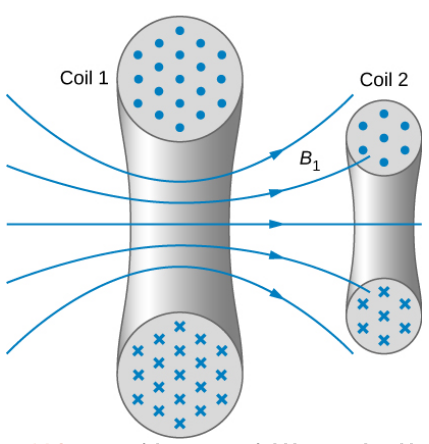
\includegraphics[width=0.5\textwidth]{figures/ind1.png}
\caption{\label{fig:ind1} The concept of mutual inductance.}
\end{figure}
\end{frame}

\begin{frame}{Mutual Inductance}
First, some notation:
\begin{itemize}
\item The flux through coil 2 by coil 1: $\phi_{21}$
\item The flux through coil 1 by coil 2: $\phi_{12}$
\end{itemize}
Mutual inductance of coil 2 with respect to coil 1:
\begin{equation}
M_{21} = \phi_{21}\frac{N_2}{I_1}
\end{equation}
Mutual inductance of coil 1 with respect to coil 2:
\begin{equation}
M_{12} = \phi_{12}\frac{N_1}{I_2}
\end{equation}
It can be shown that
\begin{equation}
\boxed{
M_{21} = M_{12}
}
\end{equation}
\end{frame}

\begin{frame}{Mutual Inductance}
What are the units of mutual inductance?   Consider the emf induced in loop 2 by loop 1:
\begin{equation}
\epsilon_2 = -\frac{d}{dt} \left( \phi_{21} N_2 \right)
\end{equation}
Substitution for the inductance gives
\begin{align}
\epsilon_2 &= -\frac{d}{dt} \left( \frac{M_{21} I_1}{N_2} N_2 \right) \\
\epsilon_2 &= - \frac{d}{dt} \left( I_1 M_{21}\right) \\
\epsilon_2 &= - M \frac{d I_1}{dt} \\
\epsilon_1 &= - M \frac{d I_2}{dt}
\end{align}
So inductance relates induced emf to current change, and has units of V s A$^{-1}$.
\end{frame}

\begin{frame}{Mutual Inductance}
\small
A coil of $N_2$ turns and radius $R_2$ surrounds a long solenoid of length $l_1$, radius $R_1$, and $N_1$ turns. (a) What is the mutual inductance of the two coils? (b) If $N_1 = 1000$, $N_2 = 20$, $R_1 = 3.0$ cm, $l_1 = 100.0$ cm, and $dI_1/dt = 150$ A/s, what is the induced emf in the surrounding coil?
\begin{figure}
\centering
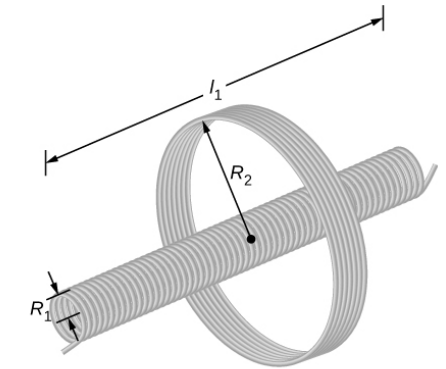
\includegraphics[width=0.5\textwidth]{figures/ind2.png}
\caption{\label{fig:ind2} Example of mutual inductance.}
\end{figure}
\end{frame}

\begin{frame}{Mutual Inductance}
\small
A current $I(t) = I_0 sin (\omega t)$ flows through the solenoid.  If $I_0 = 7.5$ A, and $\omega = 60 \pi$ rad/sec, what is the maximum induced emf in the surrounding coil?
\begin{figure}
\centering
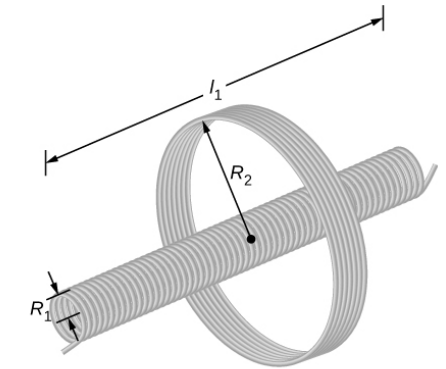
\includegraphics[width=0.5\textwidth]{figures/ind2.png}
\caption{\label{fig:ind3} Example of mutual inductance.}
\end{figure}
\end{frame}

\section{Self-inductance and inductors}

\begin{frame}{Self-inductance and inductors}
\small
\begin{figure}
\centering
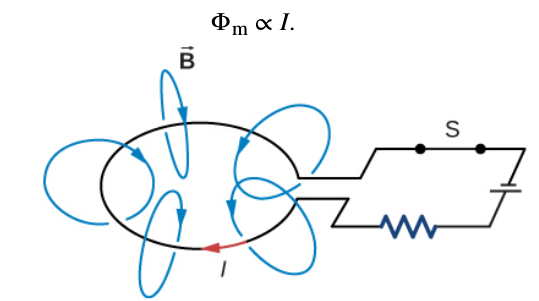
\includegraphics[width=0.35\textwidth]{figures/ind3.png} \\
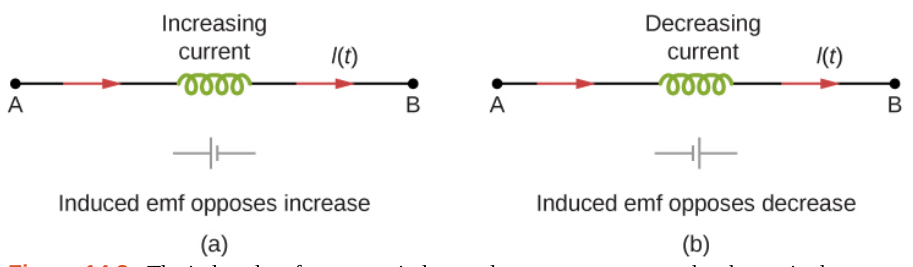
\includegraphics[width=0.65\textwidth,trim=0cm 0.1cm 0cm 0cm,clip=true]{figures/ind4.png}
\caption{\label{fig:ind4} Self-inductance in a circuit, denoted $L$, rather than $M$.}
\end{figure}
Define
\begin{align}
\epsilon &= - L\frac{dI}{dt} \\
N \phi_m &= LI
\end{align}
\end{frame}

\begin{frame}{Self-inductance and inductors}
(Observe on board): Show that the inductance of a solenoid with volume $V$ and turn density $n$ is
\begin{equation}
L = \mu_0 n^2 V
\end{equation}
\end{frame}

\begin{frame}{Self-inductance and inductors}
\begin{figure}
\centering
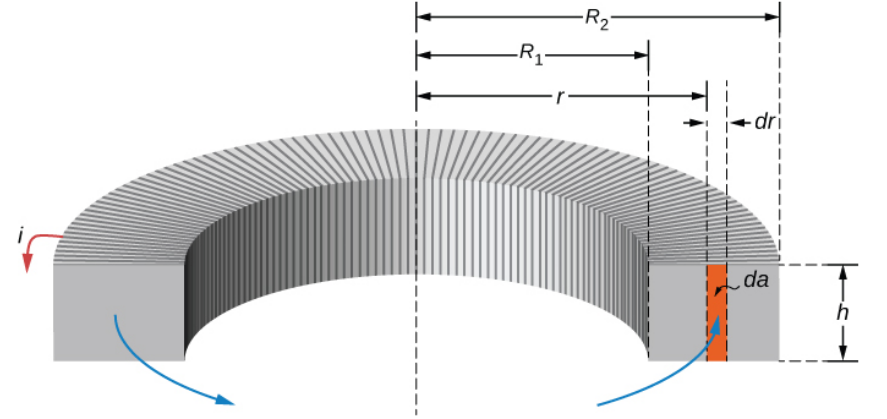
\includegraphics[width=0.7\textwidth]{figures/ind5.png}
\caption{\label{fig:ind5} A rectangular toroid.}
\end{figure}
\end{frame}

\begin{frame}{Self-inductance and inductors}
(Observe on board): Show that the inductance of a rectangular toroid as defined above is
\begin{equation}
L = \frac{\mu_0}{2\pi}N^2 h \ln\left(\frac{R_2}{R_1}\right)
\end{equation}
Thus the two expressions have turn-density squared in common, and the volume comes into play. \\
\textbf{Similar to calculating the capacitance in electrostatics.}
\end{frame}

\section{The RLC circuit}

\section{Conclusion}

\begin{frame}{Summary}
\textbf{Reading: Chapters 13 and 14} \\ \vspace{0.5cm}
\textit{This weekend:}
\begin{enumerate}
\item 13.1-2: Faraday's and Lenz's Law
\item 13.3: Motional EMF
\item 13.4: Induced E-fields
\end{enumerate}
\textit{Next week:} Chapter 14.1-3
\end{frame}

\section{Answers - Chapter 13 and Unit 4 Review}

\begin{frame}{Answers}
\small
\begin{columns}[T]
\begin{column}{0.5\textwidth}
\begin{itemize}
\item B
\item A
\item D
\item A
\item D
\item D
\item A
\item D
\end{itemize}
\end{column}
\begin{column}{0.5\textwidth}
\begin{itemize}
\item B
\end{itemize}
\end{column}
\end{columns}
\end{frame}

\section{Answers - Chapter 14}

\begin{frame}{Answers}
\small
\begin{columns}[T]
\begin{column}{0.5\textwidth}
\begin{itemize}
\item ...
\end{itemize}
\end{column}
\begin{column}{0.5\textwidth}
\begin{itemize}
\item ...
\end{itemize}
\end{column}
\end{columns}
\end{frame}

\end{document}
